%\hypertarget{estilo:capitulo}{}

\chapter{RESULTS AND DISCUSSION} \label{MatMet}
\section{Results in  the first project }
For all time windows analyzed, METEO-type words were predominant in all cases. Users' posts recurrently use in their sentences words such as rain, storm, among others. In some cases, users use the word classes METEO and HYDRO metaphorically, not referring directly to the analyzed flooding contexts.

In this context, the words were also temporally separated, and a Boxplot was plotted from the data obtained (Figure \ref{fig:my=bel}).

\begin{figure}[H]
	\centering
	\includegraphics[scale=0.5]{figs/boxplot2.png}
	\caption{Box plot, fourth time window}
	\label{fig:my=bel}
\end{figure}

Boxplot visually demonstrates the relevance of METEO class words on flood days compared to non-flood days. To prove this statistical relevance, the Mann Whitnney test was applied. 

The table \ref{table:my_} shows the statistical analysis based on the nonparametric Mann-Whitney test. For samples with a few days, the test demonstrates that the null hypothesis is not rejected, that is, evidencing that there is no statistical difference between the two series (days of flooding, not flooding). However, as the data period expands, the test shows a considerable difference between the series.

\begin{table}[H]
	\centering
	\caption{Mann-Whitney statistical results.}\label{table:my_}
	\begin{tabular}{cccc}
		\hline
		%\multicolumn{4}{c}{Mann-Whitney test (\(\alpha=0.05)\)} \\ \hline
		\multicolumn{1}{c|}{} & \multicolumn{1}{c|}{January} & \multicolumn{1}{c|}{January, February} & \begin{tabular}[c]{@{}c@{}}January, February\\ and March\end{tabular} \\ \hline
		\multicolumn{1}{c|}{Statistic of test} & \multicolumn{1}{c|}{49} & \multicolumn{1}{c|}{199} & 558 \\
		\multicolumn{1}{c|}{$p$-value} & \multicolumn{1}{c|}{0.05725} & \multicolumn{1}{c|}{0.02169} & 0.012948 \\
		\multicolumn{1}{c|}{Reject $H_0$?} & \multicolumn{1}{c|}{No} & \multicolumn{1}{c|}{Yes} & Yes \\ \hline
	\end{tabular}
\end{table}


The regions where there were more floods (Figure \ref{fig:foobar}) share similar characteristics, flat or slightly sloping regions favor the accumulation of water in the region. Large parts of flooding in urban areas occur in flat areas or with depressions and valley bottoms, usually with surface runoff hampered by the topography of the location. It can be observed that there is a particular pattern of regions where more flooding occurs within the study area, and those specific topographical characteristics of the place lead to water accumulation.

\begin{figure}[H]
	\centering
	\subfigure[R. Teixeira Leite, 227]{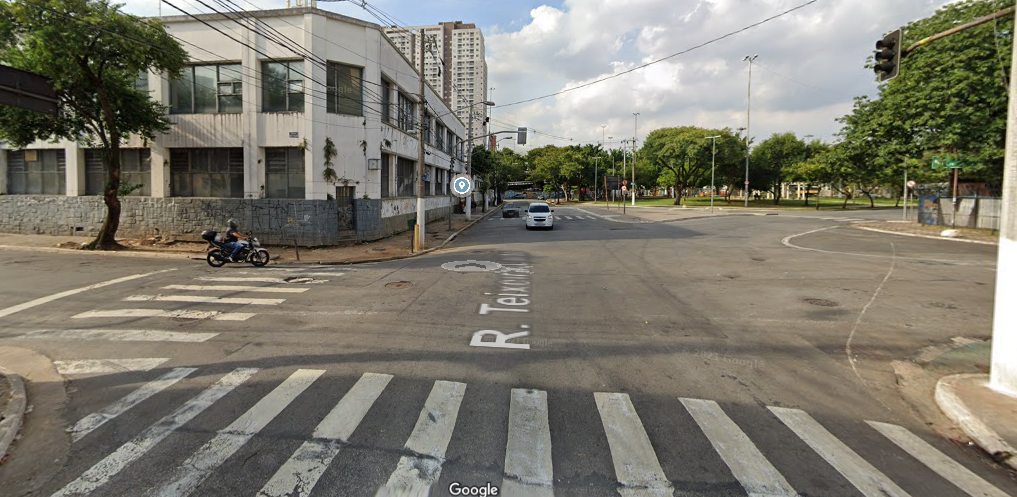
\includegraphics[width=0.35\textwidth, height=4.5cm]{figs/flood1.png}} 
	\subfigure[R. Wanderkolk, 509]{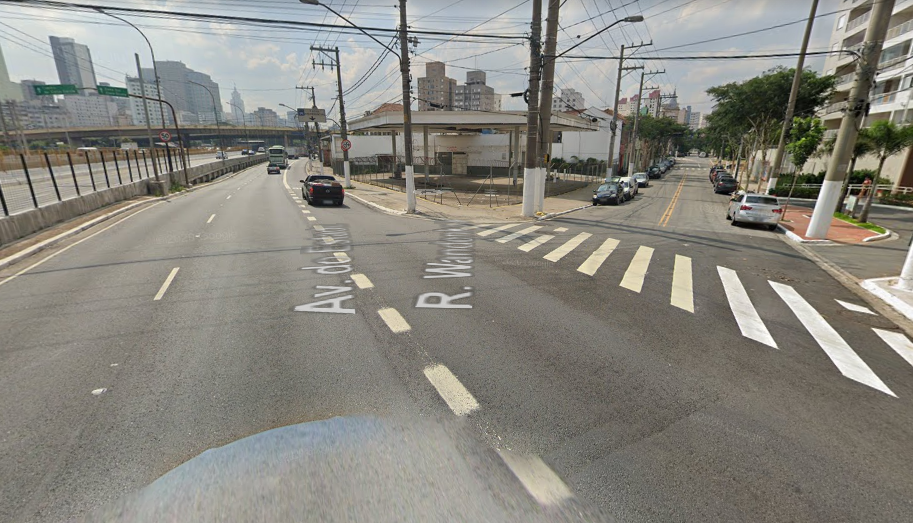
\includegraphics[width=0.35\textwidth, height=4.5cm]{figs/flood2.png}} 
	\subfigure[R. Santos Amaro, 11]{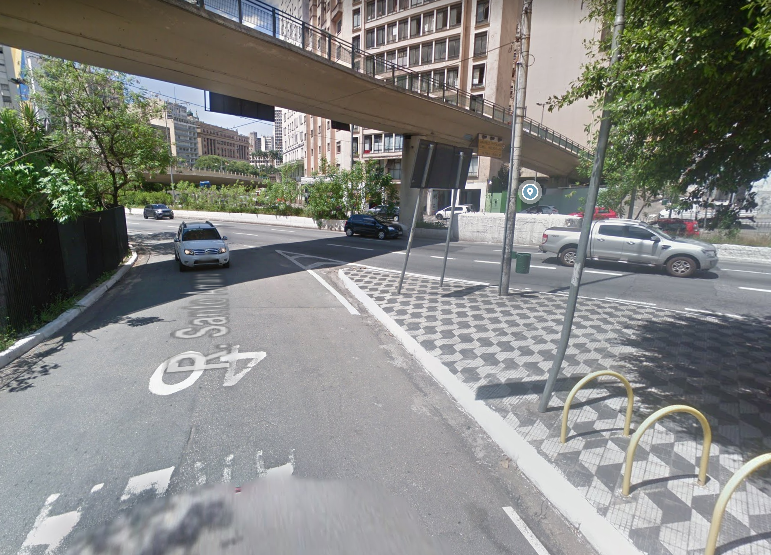
\includegraphics[width=0.35\textwidth,height=4.5cm]{figs/flood3.png}}
	\subfigure[R. Óscar Horta, 187]{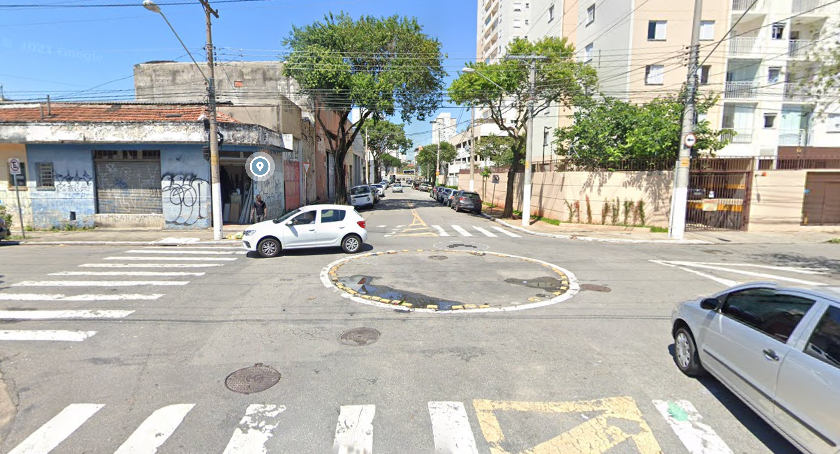
\includegraphics[width=0.35\textwidth,height=4.5cm]{figs/flood4.png}}
	\caption{Regions where more floods in the study area (Photos from Google maps)}
	\label{fig:foobar}
\end{figure}

\section{Preliminary Results in the second project}
The tweets filtered based on the words presented in the \ref{secondmethod} methodology, presented a large part of the tweets related to the context of rain and flooding. The use of other words such as 'raio' and 'tempestade', result in tweets using these words to designate a metaphorical context or with a sense displaced from the phenomena of rain and flooding. Therefore, the application of the word 'chuva' and its variations present a more stable meaning to refer to meteorological phenomena.

However, it can be observed that the filtering algorithm detects tweets using the word rain in a more poetic sense (Table \ref{table:tweets_filt}).

\begin{table}[H] \label{table:tweets_filt}
	\caption{Related and unrelated Tweets}
	\begin{tabular}{ll}
		\hline
		\multicolumn{2}{c}{Examples of Tweets}                                                                                                                                                                                                                                                                                             \\ \hline
		\multicolumn{1}{c|}{Related tweets}                                                                                                                                          & \multicolumn{1}{c}{Tweets out of context}                                                                                                           \\ \hline
		\multicolumn{1}{l|}{\begin{tabular}[c]{@{}l@{}}quem aqui gosta de pokemon?\textbackslash{}nvideo\\  de dias atras  porque a chuva estragou \\ meus planos hoje\end{tabular}} & \begin{tabular}[c]{@{}l@{}}minha força esta na solidao. não tenho\\ medo nem de chuvas tempestivas \\ nem de grandes ventanias soltas.\end{tabular} \\ \hline
		\multicolumn{1}{l|}{\begin{tabular}[c]{@{}l@{}}sabado com chuvas e minhas aluna vieram\\ fazer um alongamento para tira toda preguica\end{tabular}}                          & \begin{tabular}[c]{@{}l@{}}a ordem e seguir em frente romper a \\ tempestade e nao se ater aos ventos, raios \\ e chuvas.\end{tabular}              \\ \hline
	\end{tabular}
\end{table}

%%%%%%%%%%%%%%%%%%%%%%%%%%%%%%%%%%%%%%%%%%%%%%%%%
% The data were processed for the same time window and an exploratory data analysis was performed using the graph below (\ref{fig:graph}). The pluviometric data were collected from the 833A pluviometer, in which the accumulated rain level per day was added. This rain gauge measures the rain level  every 10 minutes. Radar precipitation data was collected in a cell that covers the same region as the pluviometer, thus processing the data for the analyzed temporal window. Tweets were collected within a radius of \si{2000 \meter} and filtered based on a list of words. The words were: 'chuva', 'chove', 'chuvoso', 'chuvosa', according to \cite{de2021effect}, these words are less spatially and temporally volatile than more local and idiosyncratic terms specifically related to the city of São Paulo (e.g. 'garoa' and 'tempestade'). 

After the unification of all attributes in a single DataFrame, a graph was plotted relating these variables to the time window studied \ref{fig:graph}.

\begin{figure}[H]
	\centering
	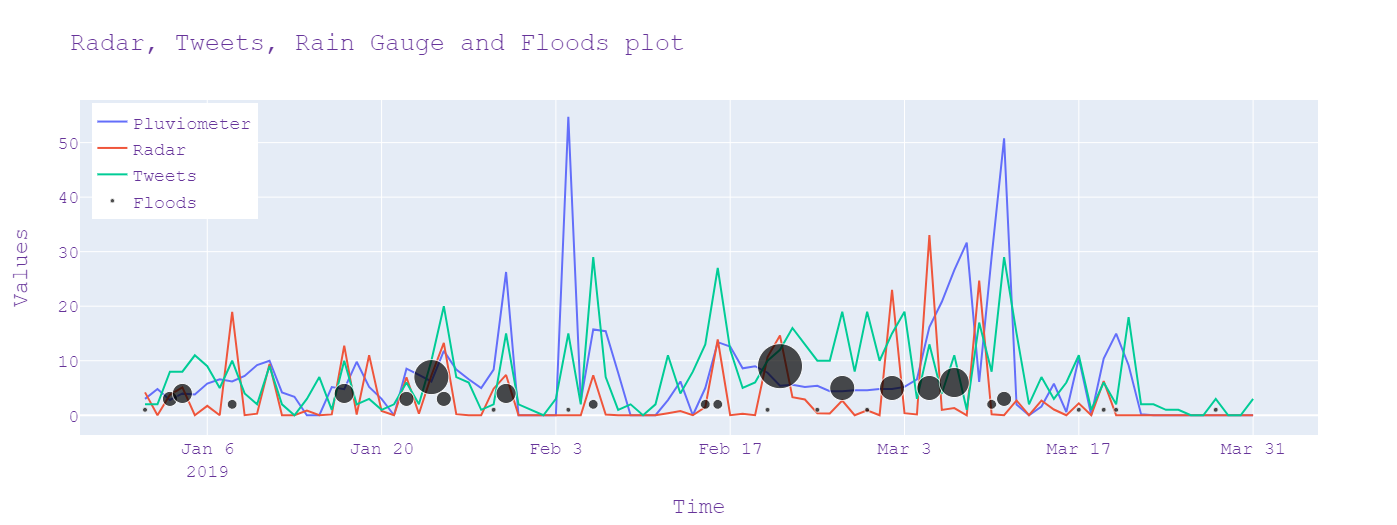
\includegraphics[width=1.2\textwidth]{figs/newplot.png}
	\caption{Plot}
	\label{fig:graph}
\end{figure}

The plotting of data indicates that on every day that flooding occurred there was an incidence of rain indicated by the rain gauge and radar and rain-related tweets. As can be seen in the figure \ref{fig:graph}, the frequency of flooding on a given day determines the size of the black circle, and that the days with the highest incidence of flooding were not peaks of rain detected by meteorological equipment.

To determine the statistical relationships a series of tests were performed. First, it was necessary to determine if the attributes were a normal distribution, so that in this way parametric or non-parametric statistical tests could be applied. For this verification, the Shapiro Wilk test was used (\ref{shapiro}).

\begin{table}[H]\label{shapiro}
	\caption{P-Values results}
	\begin{center}
	\begin{tabular}{ll}
		\hline
		\multicolumn{2}{c}{Shapiro-Wilk test $\alpha=0.05$}                              \\ \hline
		\multicolumn{1}{c|}{Attributes}      & \multicolumn{1}{c}{P-value} \\ \hline
		\multicolumn{1}{l|}{Rain Gauge}      & 7.175038015984347e-13       \\ \hline
		\multicolumn{1}{l|}{Tweet Frequence} & 2.0394061550632614e-07      \\ \hline
		\multicolumn{1}{l|}{Radar}           & 7.194410709808908e-15       \\ \hline
		\multicolumn{1}{l|}{Flood}           & 1.445436313501046e-14       \\ \hline
	\end{tabular}
\end{center}
\end{table}

In the table above \ref{shapiro}, the p-values of all attributes were below the limit of $\alpha$, discarding the null hypothesis that the distribution is normal. Based on the results, to calculate the correlations, Spearman's non-parametric test (\ref{fig:corr}) was used for these data. 

\begin{figure}[H]
	\centering
	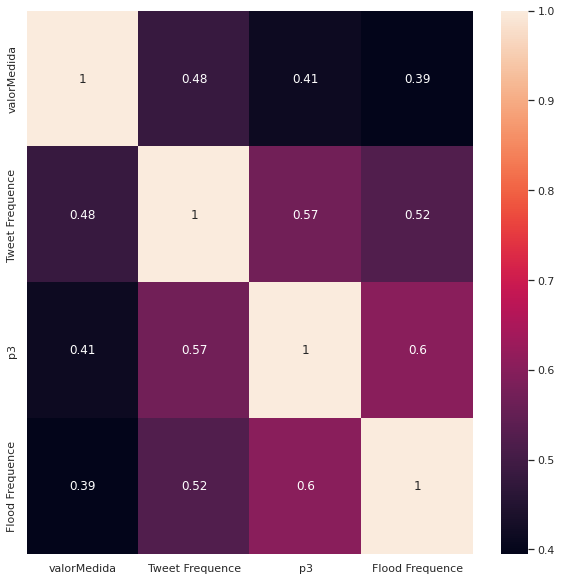
\includegraphics[width=0.47\textwidth]{figs/corr.png}
	\caption{Spearman Correlation}
	\label{fig:corr}
\end{figure}

From the correlations, it is clear that the radar (p3), followed by the tweets, have the highest correlation with the frequency of flooding and also the most significant value. According to \citen{statistics_solutions_2021}, the cited attributes indicates a strong correlation with floods. 

Furthermore, rainfall data indicate the occurrence of precipitation in opposition to Radar. As seen in figure \ref{fig:graph}, the graph indicates the low correlation between these two attributes.

From the results, the most relevant correlations will also exert greater influence on the flooding prediction.
